% vim:ft=tex

\section{Prediction on Hourly Basis}

\subsection{Data Preparation}
Since the long term goal was to predict the usage on a hourly base, some further data
transformation steps are necessary to achieve this goal. Furthermore the data records will
increase significantly on an hourly granularity. Therefore the normal use of Anaconda and Jupyter
on a local computer may be not sufficient due to low physical memory. An ideal use case for our
newly installed Hadoop cluster! There PySpark can be used as already used under Data Profiling
Part 1 in chapter \ref{dp1} to manage \glqq bg data\grqq transformations. Unfortunately the behaviour and syntax of PySpark
is sometimes a little more complicated than Pandas. For example, in PySpark it is not easily
possible to iterate over rows since the data frame is distributed over the worker nodes and thus it
only allows columnwise operations. Moreover, Pandas operations such as „iloc“ are not available
in PySpark. But the API comes also with some advantages, e.g. it is quite performant on big data
scale (i.e. it can easily perform several million of records) and it has an SQL approach.
Functions like \glqq select\grqq \glqq where\grqq and \glqq filter\grqq are syntactical close by to SQL as we know from MySQL
and other database management systems.\\\\
The structure of the weather data is inconsistent due to \glqq hourly weather\grqq  While the other columns
only contain simple values, the column \glqq hourly weather\grqq contains nested JSON lists. This means
that these nested lists must somehow become normal columns. This was a little more complicated
than expected, but not impossible. Fortunately, PySpark allows one to define \glqq schemas\grqq that are
used as a kind of blueprint by Spark to read the Spark data frame. With the following code one
can already create normal columns from the JSON lists:
\begin{figure}[H]
\hspace{-1.6cm}
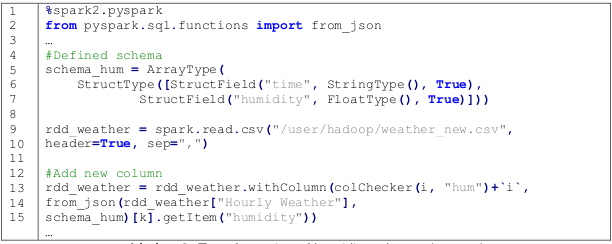
\includegraphics[width=1.2\textwidth]{img/listing5}\label{fig:listing5}
\captionof{figure}{Transformation of humidity columns (excerpt)}\label{fig:listing5}
\end{figure}
he excerpt from \ref{fig:listing5} shows that \glqq structTypes\grqq can be used to search the individual sublists
of \glqq hourly weather\grqq .
The complete script is contained in the Zeppelin notebook \glqq DFGeneration.json\grqq and can also be found on GitHub.
\\\\
The described transformation creates a new column with the corresponding value for each hour.
The script works dynamically. For example, the user can look at the data with two hours from today,
which then looks like this:
\begin{figure}[H]
\hspace{-1.6cm}
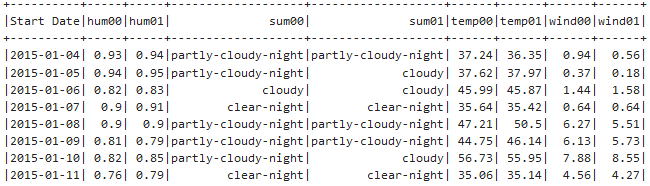
\includegraphics[width=1.2\textwidth]{img/figure7_weather_df}\label{fig:figure7_weather_df}
\captionof{figure}{Weather dataframe after transformation for two hours}\label{fig:figure7_weather_df}
\end{figure}
\subsubsection{Holidays}

To add the bank holidays are day-based, so they should be set on a 24 hour windows.
However, fixing the bank holidays from midnight to midnight the next day might not
be the best solution as people might consider the evening of a bank holiday the same
way as they do for normal week day, while the evening of the day before will be more
interesting. Indeed, when people want to go out in the evening and go to bed late,
they will prefer doing that when they don't have to wake up early in the morning,
thus they may be more likely to use a bike the end of the day before the bank
holiday than of the day itself.

This is why it might be a good idea to test the accuracy of the prediction
placing bank holidays from 6pm the day before to 6pm the day itself.

% TODO: accuracies
% The accuracy of the overall model on the testing data using the bank-holidays
% starting at 6pm is []. When not using this, we get a lower accuracy of
% [].
% TODO: RMSE ?

\subsection{Learning and Prediction}

For the learning part, we used the same algorithm as described in~\ref{data_prediction}.
We trained twenty-four models, one per future hour to predict.
For each model, we only use the past and current data which we match to
the future expected number of rented bike for the given following hour,
no other future data is used.

We used the sliding-windows hourly based data over 48 hours (aggregating per slice
of 6 hours after the first 24 hours).
We have an accuracy of 0.800638 on the test dataset.
On the graph below, you can see several randomly selected days in the testing set
starting at midnight and predicting for the whole day. The title above each graph
indicates the date displayed, the actual expected value is in red and the
predicted one is in blue.
\begin{figure}[H]
\hspace{-0.9cm}
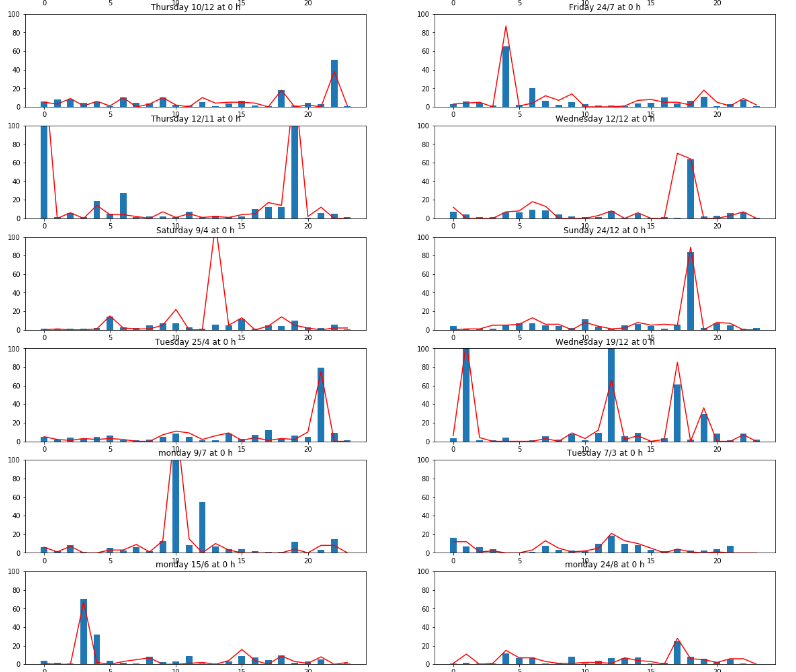
\includegraphics[width=1.1\textwidth]{img/hourly_predictions}
\captionof{figure}{Comparison of expected (red) and predicted (blue) hourly rented bikes on test dataset}\label{fig:hourly_pred}
\end{figure}

As we can see on the Figure~\ref{fig:hourly_pred} and considering the measured accuracy,
we can see that we can predict quite well the amount of rented bikes for the following
24 hours based on the data of the previous 48 hours.
